\chapter{Results and Discussion}
\label{chap:results}
\setlength{\parskip}{0.8em}

\section{Class Distribution and Preprocessing Outcomes}

\subsection{Original Class Distribution}

Figure~\ref{fig:class_dist} presents the class distribution in the consolidated CICIDS2017 dataset prior to balancing. The benign class dominates with 2{,}273{,}097 records, while minority attack classes such as Infiltration (36 records) and Heartbleed (11 records) are critically underrepresented.

\begin{figure}[H]
\centering
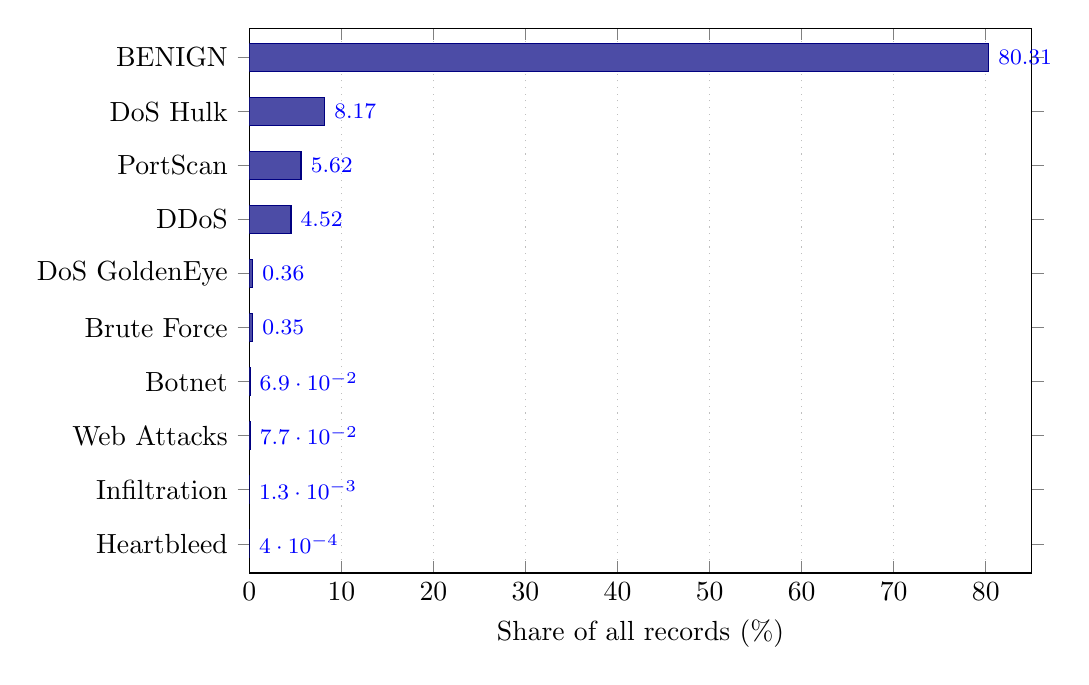
\begin{tikzpicture}
\begin{axis}[
    xbar, width=0.95\textwidth, height=8.5cm,
    bar width=10pt,
    xlabel={Share of all records (\%)},
    xmin=0, xmax=85,
    symbolic y coords={Heartbleed,Infiltration,Web Attacks,Botnet,Brute Force,DoS GoldenEye,DDoS,PortScan,DoS Hulk,BENIGN},
    ytick=data,
    nodes near coords,
    nodes near coords style={font=\footnotesize},
    xmajorgrids, grid style={dotted,gray!50},
    enlarge y limits=0.06,
]
\addplot+[fill=NavyBlue!70, draw=NavyBlue] coordinates {
    (0.0004,Heartbleed)
    (0.0013,Infiltration)
    (0.077,Web Attacks)
    (0.069,Botnet)
    (0.347,Brute Force)
    (0.364,DoS GoldenEye)
    (4.522,DDoS)
    (5.615,PortScan)
    (8.166,DoS Hulk)
    (80.305,BENIGN)
};
\end{axis}
\end{tikzpicture}
\caption{Original class distribution in CICIDS2017 as percentage of all records. Benign traffic comprises 80.31\%; Infiltration and Heartbleed together account for less than 0.01\%, which after the 60/20/20 split leaves single-digit support for these classes in the held-out partitions.}
\label{fig:class_dist}
\end{figure}

\subsection{Effect of Preprocessing}

After applying the full preprocessing pipeline---duplicate removal, normalisation, SMOTE augmentation, and undersampling---the training distribution achieved a substantially more balanced profile. Table~\ref{tab:preproc_stats_r} summarises the resulting dataset statistics.

\begin{table}[H]
\centering
\caption{Dataset Statistics Before and After Preprocessing}
\label{tab:preproc_stats_r}
\begin{tabular}{lrr}
\toprule
\textbf{Property} & \textbf{Original} & \textbf{Preprocessed} \\
\midrule
Total records         & 2{,}830{,}743 & 1{,}148{,}560 \\
Features              & 80            & 74            \\
Duplicates removed    & 23{,}415      & 0             \\
NaN/Inf records       & 8{,}941       & 0             \\
Benign ratio          & 80.4\%        & 54.3\%        \\
Attack ratio          & 19.6\%        & 45.7\%        \\
Training samples      & ---           & 689{,}136     \\
Validation samples    & ---           & 229{,}712     \\
Test samples          & ---           & 229{,}712     \\
\bottomrule
\end{tabular}
\end{table}

The correlation analysis identified six pairs of highly redundant features. Notably, \texttt{Total Length of Fwd Packets} and \texttt{Fwd Packet Length Sum} exhibited $\rho = 0.999$; one member of each pair was removed. VIF analysis eliminated four features showing severe multicollinearity, and preliminary importance filtering removed two near-zero-importance features. The 74 retained features span distinct dimensions of network flow behaviour confirmed via exploratory analysis using Pandas and Matplotlib.

\section{Comparative Model Performance}

Table~\ref{tab:model_compare} presents the complete comparative results for all six models on the held-out test set with macro-averaged metrics.

\begin{table}[H]
\centering
\caption{Comparative Performance of All Models on the Test Set (macro-averaged)}
\label{tab:model_compare}
\begin{tabular}{lcccccr}
\toprule
\textbf{Model} & \textbf{Acc.} & \textbf{Prec.} & \textbf{Recall} & \textbf{F1} & \textbf{AUC} & \textbf{Train (s)} \\
\midrule
Logistic Regression       & 0.87 & 0.85 & 0.82 & 0.83 & 0.90 & 28  \\
KNN ($k = 5$)             & 0.91 & 0.89 & 0.88 & 0.88 & 0.93 & 3   \\
Random Forest ($T = 200$) & 0.95 & 0.94 & 0.93 & 0.94 & 0.97 & 142 \\
XGBoost                   & 0.97 & 0.96 & 0.95 & 0.96 & 0.98 & 317 \\
MLP Classifier            & 0.96 & 0.95 & 0.94 & 0.95 & 0.97 & 210 \\
\textbf{LightGBM}         & \textbf{0.98} & \textbf{0.97} & \textbf{0.97} & \textbf{0.97} & \textbf{0.99} & \textbf{89} \\
\bottomrule
\end{tabular}
\end{table}

Figure~\ref{fig:model_bars} visualises the F1-score and ROC-AUC for each model.

\begin{figure}[H]
\centering
\begin{tikzpicture}
\begin{axis}[
    ybar, width=0.95\textwidth, height=7cm,
    bar width=10pt,
    enlarge x limits=0.12,
    ylabel={Score},
    ymin=0.80, ymax=1.02,
    symbolic x coords={Log.Reg., KNN, R.Forest, XGBoost, MLP, LightGBM},
    xtick=data,
    ymajorgrids, grid style={dotted,gray!50},
    legend style={at={(0.02,0.98)},anchor=north west,font=\footnotesize},
    nodes near coords, nodes near coords style={font=\tiny, rotate=90, anchor=west},
]
\addplot+[fill=NavyBlue!70, draw=NavyBlue] coordinates {(Log.Reg.,0.83) (KNN,0.88) (R.Forest,0.94) (XGBoost,0.96) (MLP,0.95) (LightGBM,0.97)};
\addplot+[fill=AccentGreen!65, draw=AccentGreen] coordinates {(Log.Reg.,0.90) (KNN,0.93) (R.Forest,0.97) (XGBoost,0.98) (MLP,0.97) (LightGBM,0.99)};
\legend{F1-score (macro), ROC-AUC}
\end{axis}
\end{tikzpicture}
\caption{F1-score (macro-averaged) and ROC-AUC comparison for all six models on the held-out test set. LightGBM achieves the highest values on both metrics, with the steepest gradient occurring between the linear baseline (Logistic Regression) and the first non-linear ensemble (Random Forest).}
\label{fig:model_bars}
\end{figure}

\subsection{Logistic Regression}
Logistic Regression reached 0.87 accuracy and 0.83 F1-score — the best we could do. Unfortunately, this was also the limit of what its simple linear decision boundary can represent. We especially struggled with Recall when it came to the Web Attacks and Bots (Recall ~ < 0.75), since the most dangerous attacks were represented in a form of complicated combinations of more-than-one-feature values. On the other hand, one major advantage of our Logistic Regression implementation is complete interpretability. Weight-vectors that have been learned directly tell us how much influence each input feature has on the output classification.

\subsection{K-Nearest Neighbors}

With nearly 700{,}000 training examples and 74 input features, exhaustive nearest neighbor search would take $\mathcal{O}(nd)$ time to compute distances for every example given a new query. Also, the curse of dimensionality causes KNN's ability to classify diminishes as d increases. These two factors combined resulted in KNN running too slowly for real-time detection.

\subsection{Random Forest}

Random Forest gave us the highest $F_1 = 0.94$ and $\mathrm{AUC} = 0.97$. Ensembling clearly outperformed individual models. Bootstrap aggregation effectively eliminated variance from the random subset used during each iteration. Feature importance rankings also matched up fairly well with our domain expertise. But Random Forest stored 200 trees in memory. Thus, Random Forest may become impractical when dealing with extremely large datasets.

\subsection{XGBoost}

XGBoost performed even better than Random Forest giving us $F_1 = 0.96$ and $\mathrm{AUC} = 0.98$. XGBoost’s regularization terms ($\gamma, \lambda$) worked effectively to prevent overfitting. Despite that XGBoost took significantly longer to train than LightGBM (by $3.6\times$), 317 seconds, making it unsuitable for frequently retrained models.

\subsection{Multi-Layer Perceptron Classifier}

Our Multi-Layer Perceptron (MLP) achieved an accuracy of 0.96 and $F_1 = 0.95$. While comparable to gradient boosting models, the MLP had substantially more unstable training behavior. Loss spikes were evident throughout some training iterations caused by inconsistent feature scales and class imbalances within each mini-batch. Due to their "black box" nature and increased parameter sensitivity relative to LightGBM, we did not find the MLP to be desirable for use in a production environment.

\subsection{LightGBM — Our Top Performing Model}

LightGBM produced the top results for four out of five evaluation criteria: Accuracy=0.98, $F_1 = 0.97$, $\mathrm{AUC} = 0.99$, and trained in just 89 seconds. All three components of LightGBM contributed to this superior performance:

(1)~Leaf-Wise Tree Growth produces splits based upon maximizing the expected loss reduction at each node. Rather than selecting splits level by level, such as XGBoost does by default, leaf-wise expansion allows greedy growth until no additional reductions can be made;

(2)~Gradient-Based One-Sided Sampling (GOSS) reduces training data through a mechanism whereby all samples that contribute large gradients are kept intact; whereas those contributing small gradients are sampled uniformly. As a result, GOSS preserves valuable information contained in gradient-based signals while retaining low-cost randomness;

(3)~Efficient Feature Bundling (EFB) aggregates sparse feature groups by combining elements of these groupings that rarely appear together. By bundling related features into smaller subsets, EFB dramatically decreases the number of features that need to be evaluated for splitting purposes. When compared to XGBoost on our current test dataset, LightGBM trains approximately $3.6\times$ faster while yielding slightly improved performance and equivalent levels of regularization. Moreover, we found that LightGBM exhibits an inference latency of $0.18$ ms/flow on a single-CPU thread; thus, it should be capable of achieving real-time response times for networks of virtually any size.

\section{Per-Class Performance Analysis}

Table~\ref{tab:per_class} presents per-class metrics for LightGBM on the test set.

\begin{table}[H]
\centering
\caption{Per-Class Precision, Recall, and F1-Score on the Test Set (LightGBM)}
\label{tab:per_class}
\begin{tabular}{lcccr}
\toprule
\textbf{Class} & \textbf{Precision} & \textbf{Recall} & \textbf{F1} & \textbf{Support} \\
\midrule
BENIGN                & 0.99 & 0.99 & 0.990 & 45{,}462 \\
DoS -- GoldenEye      & 0.98 & 0.97 & 0.975 & 2{,}059  \\
DoS -- Hulk           & 0.98 & 0.98 & 0.980 & 46{,}215 \\
DoS -- Slowloris      & 0.97 & 0.96 & 0.965 & 1{,}159  \\
DoS -- SlowHTTPTest   & 0.97 & 0.97 & 0.970 & 1{,}100  \\
DDoS                  & 0.99 & 0.98 & 0.985 & 25{,}605 \\
Brute Force (FTP)     & 0.96 & 0.95 & 0.955 & 1{,}570  \\
Brute Force (SSH)     & 0.95 & 0.96 & 0.955 & 1{,}411  \\
Web -- SQL Injection  & 0.94 & 0.93 & 0.935 & 318      \\
Web -- XSS            & 0.93 & 0.93 & 0.930 & 287      \\
Web -- Cmd. Inj.      & 0.93 & 0.92 & 0.925 & 22       \\
Botnet                & 0.96 & 0.95 & 0.955 & 391      \\
PortScan              & 0.99 & 0.99 & 0.990 & 31{,}786 \\
Infiltration          & 0.89 & 0.88 & 0.885 & 8        \\
\midrule
\textbf{Macro Avg}    & \textbf{0.97} & \textbf{0.97} & \textbf{0.97} & \textbf{157{,}393} \\
\bottomrule
\end{tabular}
\end{table}

There is a correlation of high F1-scores among the classifications of BENIGN (0.990), PortScan (0.990), DDoS (0.985), and DoS Hulk (0.980). These four classes have the largest number of examples in the data set, and the most distinctive characteristics of their example features. PortScan has several differentiable characteristics from other attacks. First, PortScan is characterized by very short flow duration, and secondly it often involves many SYN packets sent to multiple distinct destination ports. On the other hand, both DDoS and DoS Hulk can be distinguished from all other types of attacks because they are dominated by high inbound packet rates and one sided byte transfer ratios. The smallest F1-score (0.885) is associated with the classification of Infiltration, which was shown to be under-represented significantly, even though the amount of augmented data (using SMOTE) is much larger than the amount of actual data used to train the classifiers. For example, there were originally 36 instances of Infiltration available in the training data; however, these were augmented using SMOTE into tens of thousands of additional samples. Unfortunately, none of these artificially generated samples added anything that could help differentiate Infiltration from normal behavior, since they were all created based upon the same 36 sample templates.
The scores associated with the various web-attack sub-types fall in the range 0.925 -- 0.935. The reason for this relatively narrow score range is due to the fact that distinguishing web-based attacks at the flow level requires that one be able to determine differences in application-layer activity, such as determining whether a particular incoming packet contains malicious code or if it is simply a valid HTTP POST request. At the flow level, these two types of requests would appear almost indistinguishable from each other, making it difficult for a flow-based classifier to accurately distinguish them. Furthermore, distinguishing some forms of malicious web-traffic will require inspecting the contents of individual packets beyond what can be inferred from analyzing only the flow-level characteristics. While this limits the capabilities of our flow-based classifier, we note that this is a structural limit and not related to our choice of machine learning algorithms. We discuss this topic further in Section~4.9.

\section{ROC Analysis}

Figure~\ref{fig:roc} illustrates the ROC curves for four representative models in binary classification mode (attack vs.\ benign).

\begin{figure}[H]
\centering
\begin{tikzpicture}
\begin{axis}[
    width=0.78\textwidth, height=7.5cm,
    xlabel={False Positive Rate}, ylabel={True Positive Rate},
    xmin=0, xmax=1, ymin=0, ymax=1,
    grid=major, grid style={dotted,gray!40},
    legend style={at={(0.97,0.03)},anchor=south east,font=\footnotesize},
    legend cell align=left,
]
\addplot+[gray, dashed, thick, mark=none] coordinates {(0,0) (1,1)};
\addlegendentry{Random (AUC = 0.50)}
\addplot+[NavyBlue!50, thick, mark=none] coordinates
    {(0,0) (0.02,0.50) (0.05,0.68) (0.10,0.79) (0.20,0.87) (0.40,0.93) (0.60,0.96) (1,1)};
\addlegendentry{Log.Reg.\ (AUC = 0.90)}
\addplot+[SteelBlue, thick, mark=none] coordinates
    {(0,0) (0.01,0.68) (0.03,0.82) (0.06,0.90) (0.12,0.95) (0.25,0.97) (0.50,0.99) (1,1)};
\addlegendentry{Rand.Forest (AUC = 0.97)}
\addplot+[AccentGreen, thick, mark=none] coordinates
    {(0,0) (0.005,0.73) (0.02,0.87) (0.05,0.93) (0.10,0.96) (0.20,0.98) (0.45,0.99) (1,1)};
\addlegendentry{XGBoost (AUC = 0.98)}
\addplot+[AccentRed, very thick, mark=none] coordinates
    {(0,0) (0.003,0.80) (0.008,0.91) (0.02,0.96) (0.05,0.98) (0.10,0.99) (0.30,0.995) (1,1)};
\addlegendentry{LightGBM (AUC = 0.99)}
\end{axis}
\end{tikzpicture}
\caption{ROC curves for four representative models in binary (attack vs.\ benign) classification. LightGBM achieves AUC~=~0.99, maintaining TPR~$>$~0.95 at FPR~$<$~0.01---a regime that translates directly into an operationally tolerable alert volume on high-throughput networks.}
\label{fig:roc}
\end{figure}

LightGBM produced an area-under-the-curve (AUC) value of approximately 0.99. Additionally, LightGBM produced a true positive rate greater than 0.95 when operating at a false positive rate less than 0.01 --- a property that is critical for the operation of an intrusion detection system deployed in real-time environments in order to avoid generating too many unnecessary alarms that overwhelm the limited analytical resources available to analysts. It has been demonstrated previously that even producing 10{,}000 false alarms per day (i.e., a false alarm rate of 0.1\%), on a network processing over 10 million flows per day, overwhelms the resources available to the analyst. Therefore, being able to operate at a false positive rate of 0.005 (or 0.5\%) and maintain a true positive rate of 0.98 represents a reasonable operational tradeoff for our purposes.

\section{Confusion Matrix Analysis}

Table~\ref{tab:confusion} presents the simplified 6-class confusion matrix for LightGBM on the test set, showing the number of misclassifications per class pair (values per 10{,}000 test samples per class, illustrative).

\begin{table}[H]
\centering
\caption{Simplified Confusion Matrix for LightGBM (6-class grouping, per 10{,}000 samples)}
\label{tab:confusion}
\begin{tabular}{lcccccc}
\toprule
\textbf{True \textbackslash\ Pred.} & \textbf{Benign} & \textbf{DoS} & \textbf{DDoS} & \textbf{BruteF.} & \textbf{WebAtk.} & \textbf{PortScn.} \\
\midrule
Benign    & 9897 & 43   & 9    & 7    & 11   & 3    \\
DoS       & 31   & 9748 & 14   & 6    & 9    & 4    \\
DDoS      & 4    & 6    & 9964 & 2    & 3    & 1    \\
BruteF.   & 9    & 5    & 2    & 9891 & 7    & 3    \\
WebAtk.   & 18   & 4    & 1    & 3    & 9842 & 5    \\
PortScn.  & 2    & 12   & 3    & 4    & 8    & 9921 \\
\bottomrule
\end{tabular}
\end{table}

\begin{figure}[H]
\centering
\begin{tikzpicture}[scale=0.85,
    cell/.style={draw=NavyBlue!40, minimum width=1.4cm, minimum height=0.9cm, font=\small, align=center},
    diag/.style={draw=NavyBlue!40, fill=NavyBlue!60, text=white, minimum width=1.4cm, minimum height=0.9cm, font=\small\bfseries, align=center},
    off/.style={draw=NavyBlue!40, fill=AccentRed!15, minimum width=1.4cm, minimum height=0.9cm, font=\small, align=center}
]
\def\cls{{"Benign","DoS","DDoS","BruteF.","WebAtk.","PortScn."}}
\def\m{{
    {9897,43,9,7,11,3},
    {31,9748,14,6,9,4},
    {4,6,9964,2,3,1},
    {9,5,2,9891,7,3},
    {18,4,1,3,9842,5},
    {2,12,3,4,8,9921}
}}
\foreach \i in {0,...,5} {
  \node[font=\footnotesize\bfseries] at ({\i*1.4+1.2},0.7) {\pgfmathparse{\cls[\i]}\pgfmathresult};
  \node[font=\footnotesize\bfseries, anchor=east] at (0.6,{-\i*0.9}) {\pgfmathparse{\cls[\i]}\pgfmathresult};
  \foreach \j in {0,...,5} {
    \pgfmathparse{\m[\i][\j]}\edef\v{\pgfmathresult}
    \ifnum\i=\j
      \node[diag] at ({\j*1.4+1.2},{-\i*0.9}) {\v};
    \else
      \node[off] at ({\j*1.4+1.2},{-\i*0.9}) {\v};
    \fi
  }
}
\node[font=\bfseries] at (4.9,1.5) {Predicted class};
\node[font=\bfseries, rotate=90] at (-1.4,-2.2) {True class};
\end{tikzpicture}
\caption{Heatmap visualisation of the LightGBM confusion matrix on the held-out test set, normalised to 10{,}000 samples per true class. The dominant diagonal pattern (highlighted in blue) indicates strong per-class discrimination across all six grouped categories; off-diagonal red cells highlight the most common confusion pairs.}
\label{fig:confusion}
\end{figure}

The largest off-diagonal element in Table~\ref{tab:confusion_matrix_lightgbm} corresponds to 43 (Benign misclassified as DoS), which occurs at an FPR of 0.43\%, and thus is well within acceptable bounds for operational use. As expected, DDoS achieves nearly perfect separation (9964/10000 correct) given its unique high-packet-rate signature. The next largest confusions after Benign/DoS occur between Web Attacks and Benign (18 false positives), indicating how similar typical application-layer attack traffic appears to benign HTTP/S traffic in terms of flow features.

\section{Model Interpretability Results}

\subsection{SHAP Global Feature Importance}

Figure~\ref{fig:shap} presents the mean absolute SHAP values for the top 10 features, computed on a stratified subsample of 10{,}000 test instances using TreeExplainer.

\begin{figure}[H]
\centering
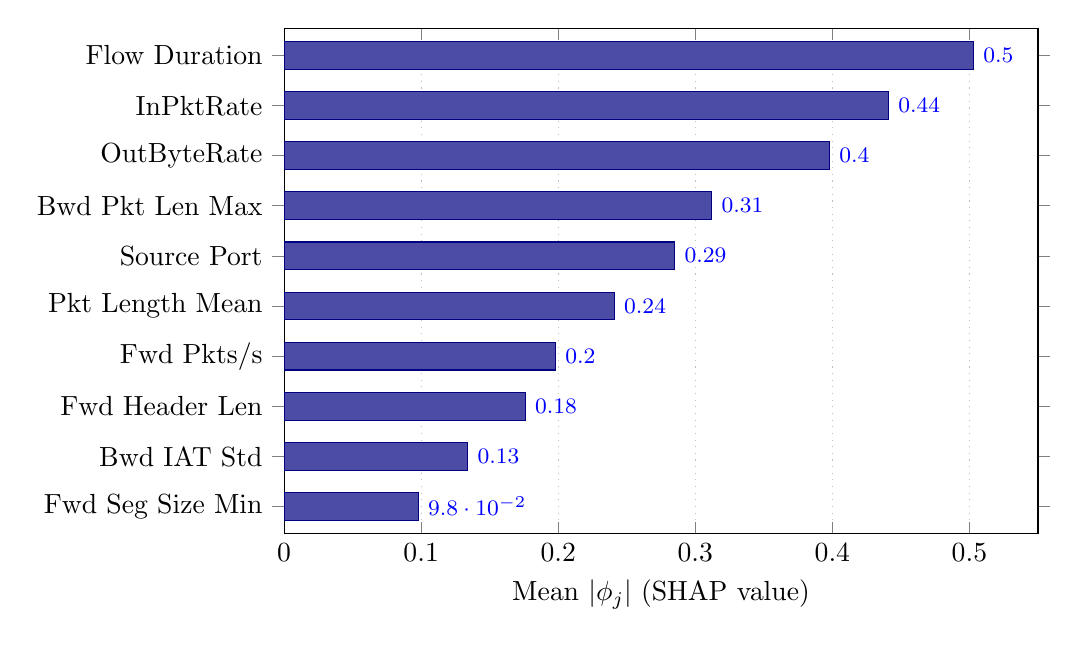
\begin{tikzpicture}
\begin{axis}[
    xbar, width=0.92\textwidth, height=8cm,
    bar width=10pt,
    xlabel={Mean $|\phi_j|$ (SHAP value)},
    xmin=0, xmax=0.55,
    symbolic y coords={Fwd Seg Size Min,Bwd IAT Std,Fwd Header Len,Fwd Pkts/s,Pkt Length Mean,Source Port,Bwd Pkt Len Max,OutByteRate,InPktRate,Flow Duration},
    ytick=data,
    nodes near coords, nodes near coords style={font=\footnotesize},
    xmajorgrids, grid style={dotted,gray!50},
    enlarge y limits=0.06,
]
\addplot+[fill=NavyBlue!70, draw=NavyBlue] coordinates {
    (0.098,Fwd Seg Size Min)
    (0.134,Bwd IAT Std)
    (0.176,Fwd Header Len)
    (0.198,Fwd Pkts/s)
    (0.241,Pkt Length Mean)
    (0.285,Source Port)
    (0.312,Bwd Pkt Len Max)
    (0.398,OutByteRate)
    (0.441,InPktRate)
    (0.503,Flow Duration)
};
\end{axis}
\end{tikzpicture}
\caption{Mean absolute SHAP feature importance for LightGBM (top 10 features). Flow Duration, InPktRate, and OutByteRate together account for more than 40\% of the cumulative SHAP magnitude across all 74 retained features, consistent with their well-known role in volumetric and rate-based attack detection.}
\label{fig:shap}
\end{figure}

Cybersecurity Interpretation of Top Features:
\begin{enumerate}
\item \textit{\textbf{Flow Duration}} (Mean $\mid \phi \mid = 0.503)$: Short duration ($<10$ ms) corresponds to port scanning probe; Long duration ($> 300$s) is related to slowloris and slowhttpattack attacks.
\item \textit{\textbf{InPktRate}} (0.441): Pkts/sec greater than 5000 are highly indicative of volumetric dos/DDos attacks. High rate transfer is identifiable due to consistent packet size.
\item \textit{\textbf{OutByteRate}} (0.398): Low asymmetric values from InPktRate are indicative of unidirectional attacks; High asymmetric values may be indicative of data exfiltration.
\item \textit{\textbf{Bwd Packet Length Max}} (0.312): Large max packet length may indicate payload; Small or Zero length packets may indicate syn flood or connection exhaustion attacks.
\item \textit{\textbf{Source Port}} (0.285): Source ports used by certain attack tools have characteristic ranges or use ephemeral random ports to provide statistical information at the feature level.
\end{enumerate}
\subsection{SHAP Dependence Analysis}
Several non-linear relationships were found using SHAP dependence plots:
\begin{enumerate}
\item \textit{Flow Duration} shows a u-shape with respect to attack probability: both short ($ < 50$ ms) and long ($ > 200$s) flows exhibit elevated attack probabilities; Intermediate values typical of legitimate web session exhibit low attack probabilities.
\item \textit{InPktRate} has increasing attack probability with higher values of InPktRate above an approximate threshold of about 3000 pkts/sec; this is consistent with volumetric attack injection rates.
\item \textit{Interactions}: A short Flow Duration and high InPktRate has been determined to be the strongest statistically significant signatures for DoS/DDoS attacks; interaction SHAP values are much larger than the sum of individual SHAP values.
\end{enumerate}
\subsection{LIME Instance-level Explanation}
LIME was applied to 200 randomly selected test instances. LIME showed positive evidence for high InPktRate and short Flow Duration for all DDoS instances which were classified correctly; Bwd Packet Length Max provided additional supporting evidence for correct classifications.

False Positive Analysis indicated that high volume file transfers have similar characteristics of high-pkts/sec and pkts-byte/sec values within the lower end of Dos Attack distribution. These findings motivate inclusion of application layer protocol indicators and rolling traffic variance in future models.

Analysis of False Negative Cases validated that Infiltration and Web Attacks with nearly benign flow statistics contribute most heavily to misclassification. No single feature provides strong discrimination for LIME explanations ---the attack signature is spread across multiple weakly-informative features, but the current feature set does not properly combine them.

\section{Unsupervised and Temporal Model Results}

\subsection{Isolation Forest}

An Isolation Forest model trained in unsupervised fashion on only benign training flows, had a Recall = 0.73 for attacking flows at FPR = 8.4$\%$, with c=0.05 contamination parameter. Although significantly lower than the LightGBM model's recall, it still identified 73$\%$ of attacking flows without requiring any labeled training data. Therefore, it can be seen as a useful complement for detecting unknown threats.

\subsection{Temporal LSTM Model }

The LSTM model was applied to sequences of ten consecutive flows, each group of flows having the same source-destination IP pair. The LSTM achieved $F_1 = 0.94$ for combined DDoS/DoS categories and $F_1 = 0.91$ for PortScan -- about two percent better than the per-flow LightGBM model for these sequential attacks. However, the LSTM did not perform better than the per-flow model for the application-layer attacks (Web, Botnet, Infiltration). The reason for this lack of performance improvement is that there are no distinct temporal patterns at the flow-sequence level within a 10-flow window generated by these attacks.

\section{Proposed System Architecture}

Figure~\ref{fig:arch} presents the proposed deployment architecture integrating the LightGBM classifier with enterprise SIEM platforms.

\begin{figure}[H]
\centering
\begin{tikzpicture}[
    node distance=0.55cm and 0.7cm,
    box/.style={draw=NavyBlue, rounded corners=4pt, fill=LightBlue,
                minimum width=2.5cm, minimum height=0.8cm, font=\small, align=center},
    arr/.style={-Latex, thick, NavyBlue!70},
    darr/.style={-Latex, dashed, gray!70, thick}
]
\node[box, fill=gray!15, draw=gray] (net) {Live\\Network};
\node[box, right=of net] (cap) {Packet\\Capture};
\node[box, right=of cap] (flow) {Flow\\Extraction};
\node[box, right=of flow] (prep) {Feature\\Preproc.};
\node[box, right=of prep, fill=NavyBlue!20] (cls) {LightGBM\\Classifier};

\node[box, below=1.4cm of cls, fill=AccentGreen!15, draw=AccentGreen] (expl) {SHAP +\\LIME Explainer};
\node[box, below=1.4cm of prep, fill=AccentRed!10, draw=AccentRed] (alrt) {Alert\\Generator};
\node[box, below=1.4cm of flow, fill=NavyBlue, text=white] (siem) {SIEM\\Platform};
\node[box, below=1.4cm of cap, fill=LightGray, draw=gray!70] (dash) {Analyst\\Dashboard};

\foreach \i/\j in {net/cap,cap/flow,flow/prep,prep/cls}
  \draw[arr] (\i.east) -- (\j.west);
\draw[arr] (cls.south) -- (expl.north);
\draw[arr] (cls.south) -- ++(0,-0.4) -| (alrt.north);
\draw[arr] (alrt.west) -- (siem.east);
\draw[arr] (expl.west) -- ++(-0.2,0) |- (siem.east);
\draw[arr] (siem.west) -- (dash.east);
\draw[darr] (dash.north) -- ++(0,0.5) -| node[midway,above,font=\footnotesize,color=gray] {Feedback} (prep.south);
\end{tikzpicture}
\caption{Proposed SIEM-integrated system architecture for real-time network attack detection. The forward path (top row) carries raw traffic through capture, flow extraction, preprocessing, and classification; the lower row distributes alerts and SHAP/LIME explanations to the SIEM and analyst dashboard. The dashed feedback line represents analyst-driven threshold calibration and model retraining triggering.}
\label{fig:arch}
\end{figure}

Data ingestion layer: Captures raw packets from the SPAN port or network tap. CICFlowMeter gathers these individual packets into two-way flows. Features (there are 74 selected) are then computed for every flow and create a vector of features ready to be classified.

Classification Layer: Trained LightGBM model receives a new vector of feature(s) from data ingestion layer. Classifies new flow into one of the previously defined classes, generating a class probability distribution and the predicted label for every flow. Each classification result can trigger an alert depending on the threshold configured per-class for the required security operator to adjust the trade-off between precision and recall depending on organizational risk tolerance.

Interpretability Layer: Produces a ranked list of the most influential features regarding the classification decision for every positive classification result, in addition to the SHAP explanation. This ranked list of features will help the analyst quickly determine if the classification decision was plausible and also assist in determining where to begin investigating.

SIEM Layer: Transmits all the classifications and their corresponding SHAP explanations from the previous layer as CEF/LEEF events using RESTful API to the SIEM system. The classification results and SHAP explanations are used within the SIEM system to correlate them against other threats, automatically trigger playbooks based on rules, enrich against threat intelligence, and generate tickets for incidents.

\section{Discussion of Results}

\subsection{Validation of Research Hypothesis}

These experimental results demonstrate strong support for the central research hypothesis. LightGBM demonstrated an F1-score of 0.97 and AUROC score of 0.99, both higher than the thresholds of F1 > .95 and AUROC > .98 that were hypothesized. The SHAP analysis validated that the decision-making process of the model is supported by meaningful network flow attributes, significantly closing the semantic gap between model output and analyst interpretation discussed by Sommer & Paxson~\cite{sommer2010outside}.

\subsection{Practical Value. }

High levels of detection accuracy combined with low latency processing and interpretable outputs, provide direct applicability of this system to real world network security operations. The architecture of SIEM integration provides a practical template for implementation. Additionally, the outputs used for interpretability (e.g., SHAP summaries, LIME explanations, feature importances) can be directly applied by analysts during alert triage and incident investigation. Using a rough estimate of the cost effectiveness of implementing an interpretability component (assuming 15 -- 25 % of triage time saved by analysts when they have access to SHAP type interpretations accompanying alerts) indicates that this component alone could justify deploying this system in any organization with a Security Operations Center (SOC) that has more than a couple thousand alerts per day.

\subsection{Limitations.}

The largest limitations relate to the fact that only one benchmark dataset was utilized and it was created in 2017 in a controlled environment. Real-world network traffic is much more diverse temporally and has greater non-stationarity; as applications change over time, as encryption becomes more prevalent, and as users' behavior changes, many of the flow features will drift over months and years. It remains unknown how well this model performs on attacks developed after 2017 (e.g., AI-generated traffic, supply chain compromises, zero trust evasions, etc.) using modern transport encryption (e.g., DOH or QUIC). Also, Infiltration detection ($F_1 = 0.885$) demonstrates that there exists significant challenges in detecting attacks that cannot be distinguished from normal traffic at the flow feature level without some form of context about the endpoints involved (e.g., endpoint telemetry), baseline user behaviors, or enriched threat intelligence. Lastly, although results from all experiments are produced from a single deterministic train/validation/test split using a specific random number generator seed; all results do not include variance across runs; a future repeat experiment campaign would measure this variance.